\part*{Appendix}
\addcontentsline{toc}{chapter}{Appendix}
\renewcommand{\thesection}{\roman{section}}
\renewcommand{\theequation}{\arabic{equation}}
\section*{Appendix One: Consumer Application}\label{section:Appendix One: Consumer Application}

The Interdisciplinary Project consists of two parts. The first one is the scientific paper in the pages before. The second part is a consumer application which will be described below.\newline
The aim of the application is to give the person who just placed an order detailed  information about the delivery. This includes the current step in the delivery process, the current position of the driver on a map and the estimated time to delivery. After successful delivery to the customer, she will be able to rate her level of satisfaction.\newline
The moment the customer finishes placing an order the backend will create an account for the customer. The credentials for the new user will be sent to the customer by email. The email directs to the application in the Play Store where it can be downloaded. This part has to be implemented in the backend once it will be used in a real scenario.\newline
\begin{figure}[htp]

\centering
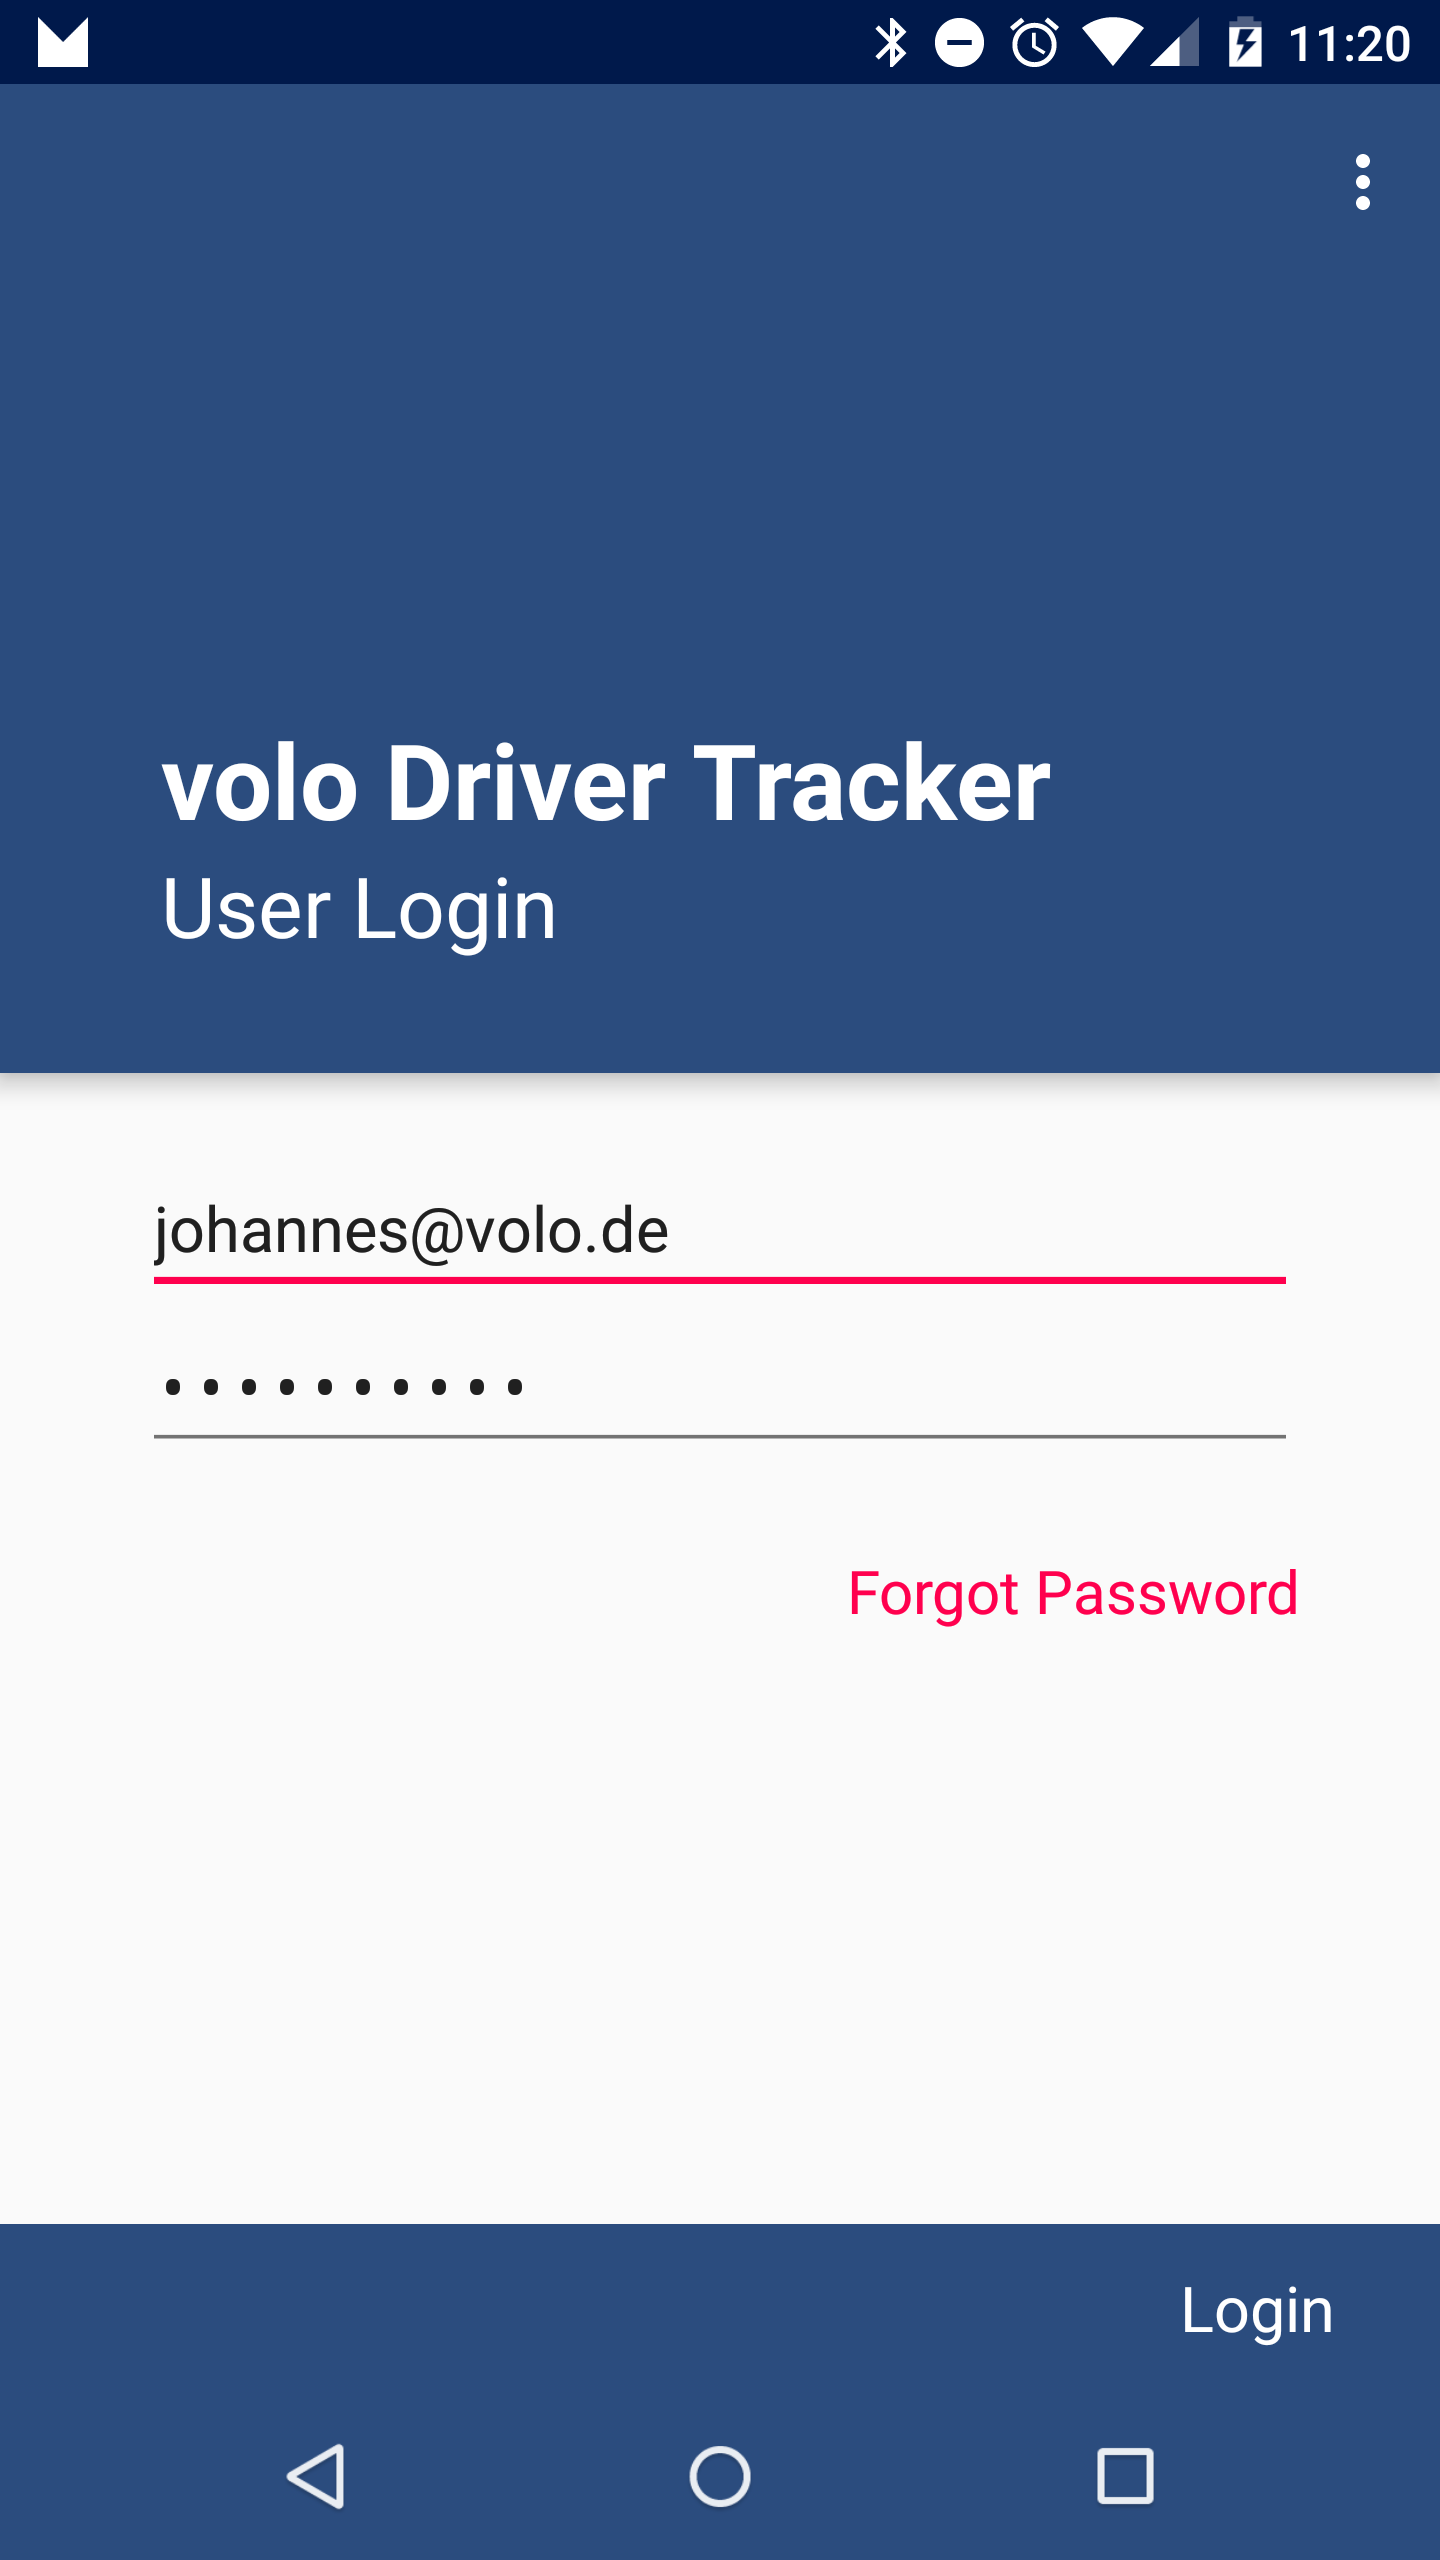
\includegraphics[width=.3\textwidth]{images/1_login.png}\hfill
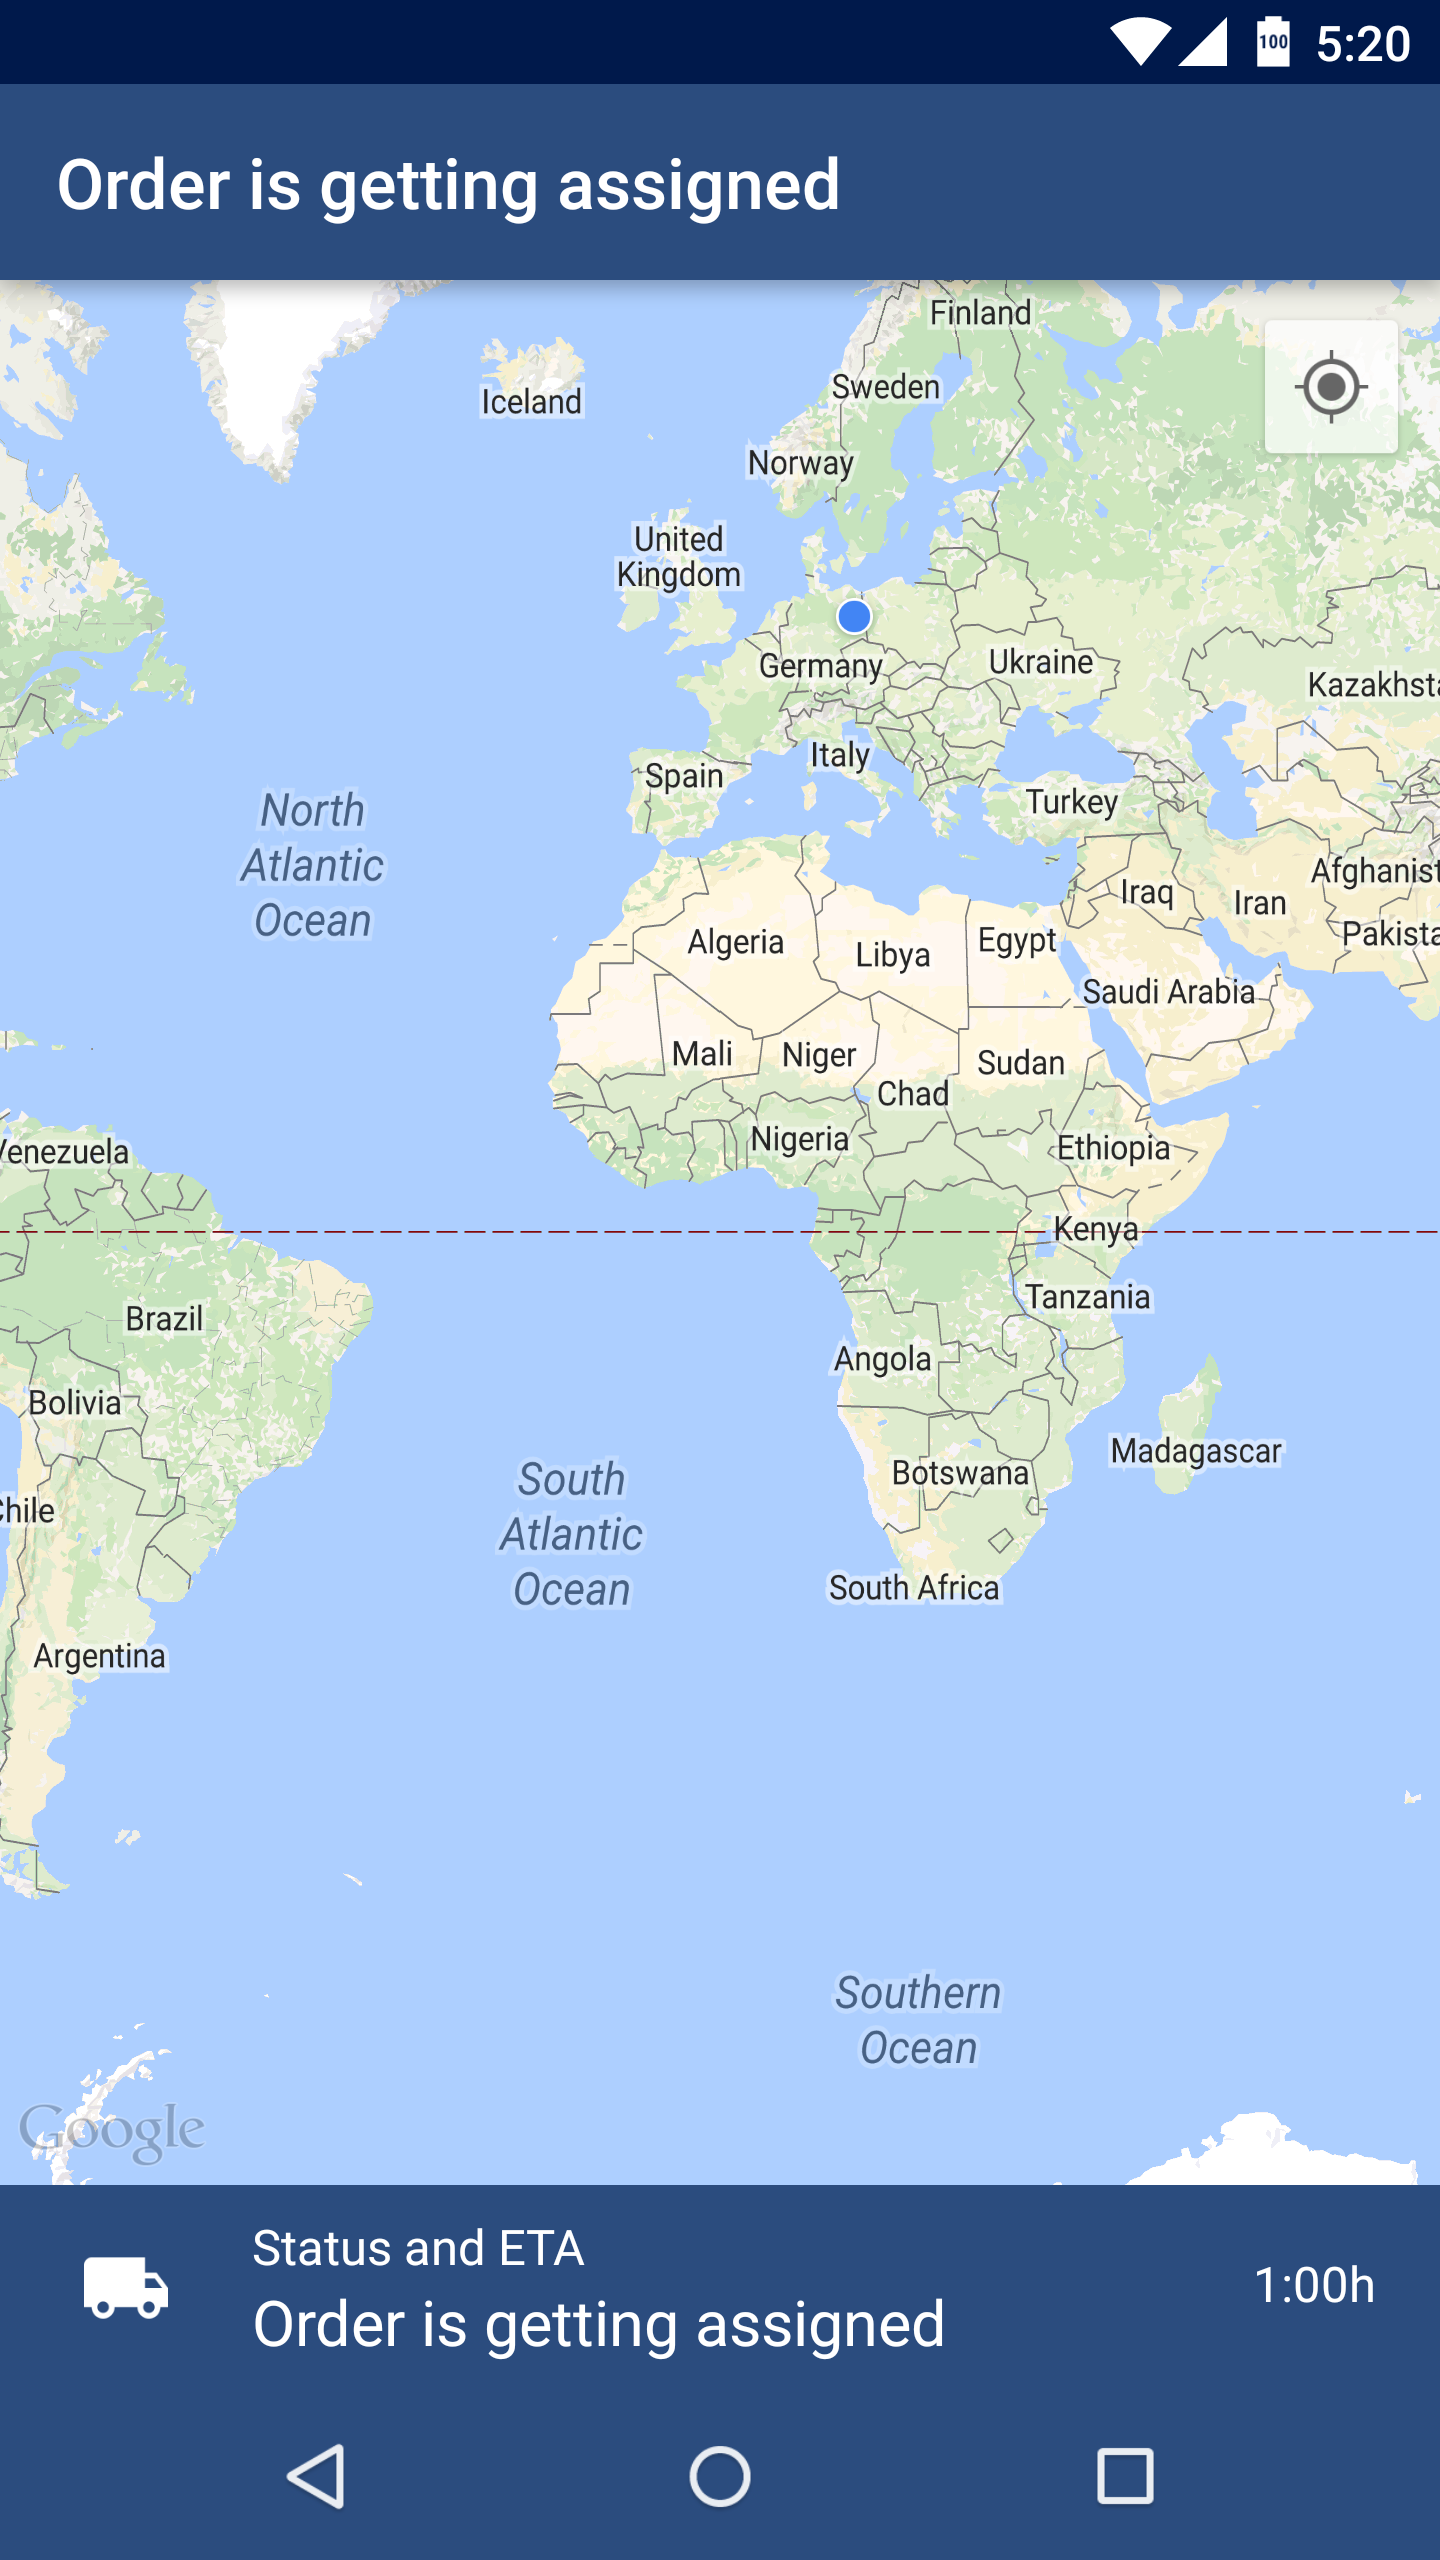
\includegraphics[width=.3\textwidth]{images/6_assign.png}\hfill
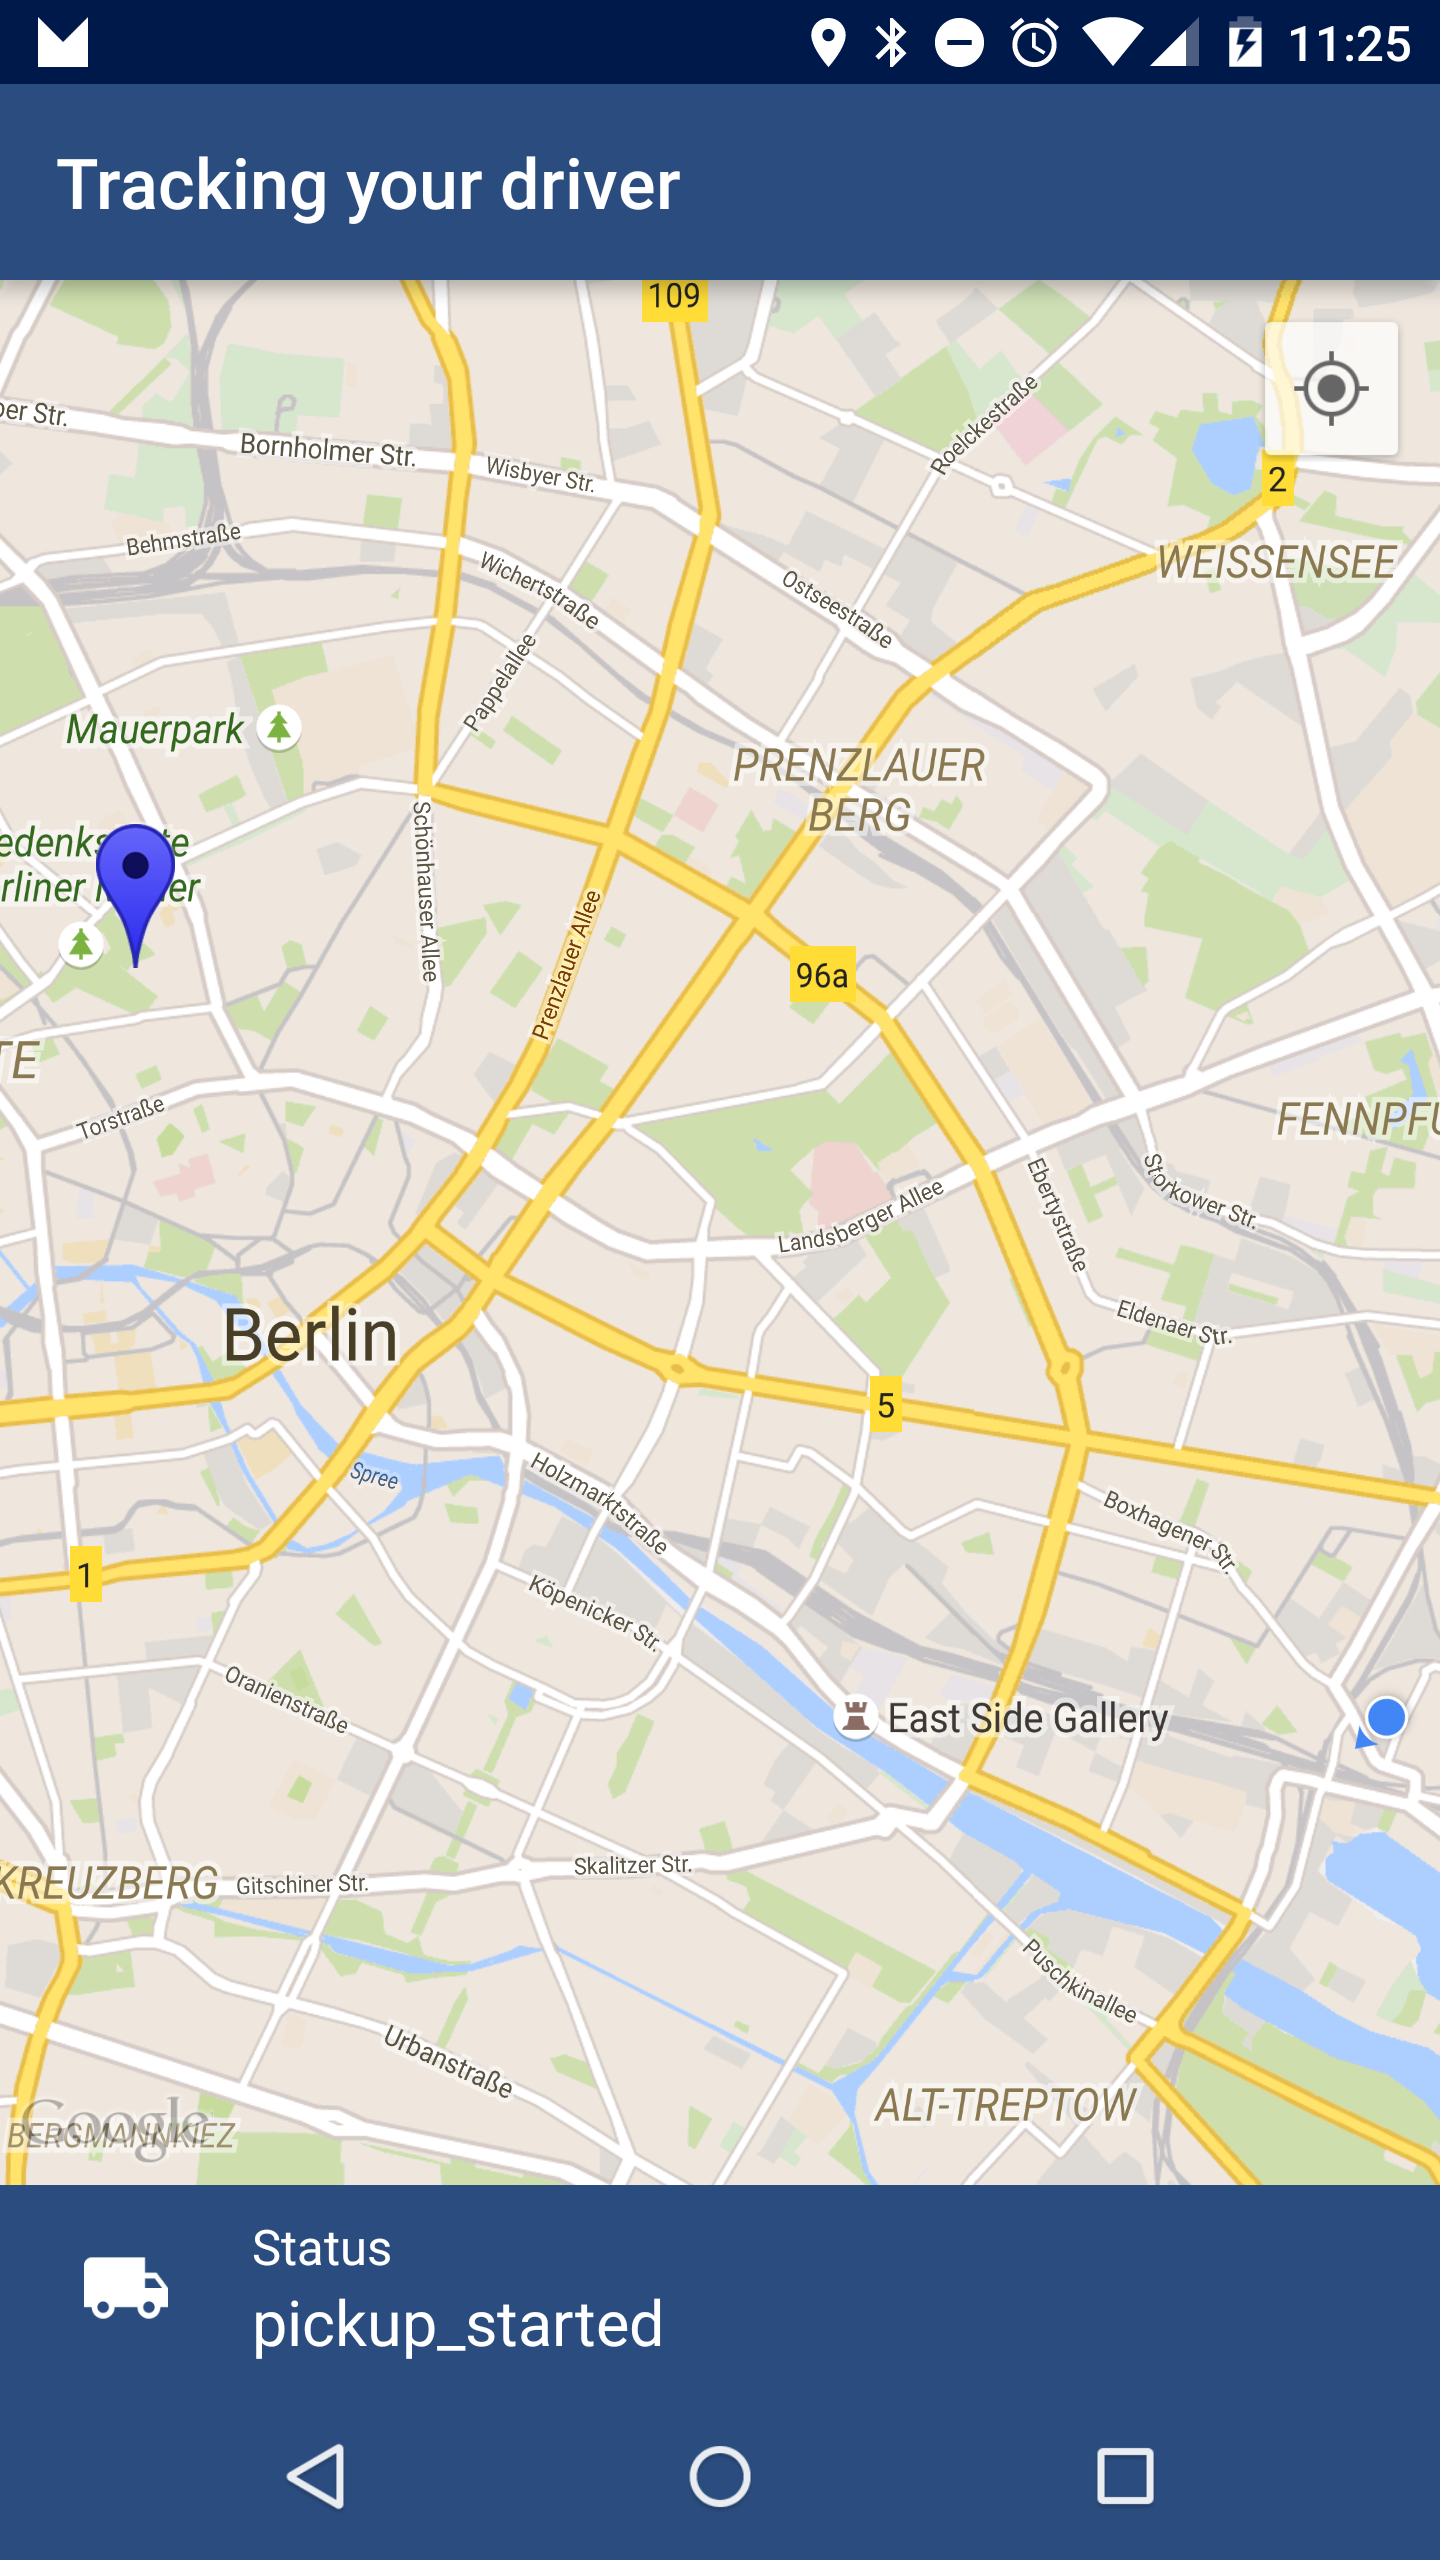
\includegraphics[width=.3\textwidth]{images/2_pickup_started.png}
\caption{The consumer application. Login on the left. Driver has to be assigned in the middle. Delivery pick up has started on the right.}
\label{fig:consumer_application}

\end{figure}
Once downloaded, the user can login into the application (Fig. \ref{fig:consumer_application}, left) by entering her user data. Since the backend does not support users seeing a driver's order, the driver account is used to demonstrate the functionality, \newline
When the customer enters the application, the screen in the middle of Figure \ref{fig:consumer_application} is shown. If the assignment of the driver hasn't happened by the time the user logs in, the driver cannot be tracked yet and the delivery time is shown as one hour.\newline
The application queries every 10 seconds for a status change on the server. As soon as the driver has accepted the order the status switches to \texttt{Driver is on the way to the Restaurant} (Figure \ref{fig:consumer_application}, right). From now on, the position of the driver is updated every 10 seconds so the customer using the application always sees where her delivery is at the moment. The customer sees the different steps of the delivery process, namely \texttt{pickup\_ended}, when the driver has entered the restaurant, and \texttt{delivery\_started}, when the driver has left the restaurant with the meal (Figure \ref{fig:consumer_application2}, left and middle). The information for the estimated time of delivery is taken from the server. It consists of the predicted preparation time, which was calculated in the scientific paper and the driving time Google Maps suggests for the route. A buffer is added to lower the customer's expectation and positively delight her be an earlier delivery.


\begin{figure}[h]

\centering
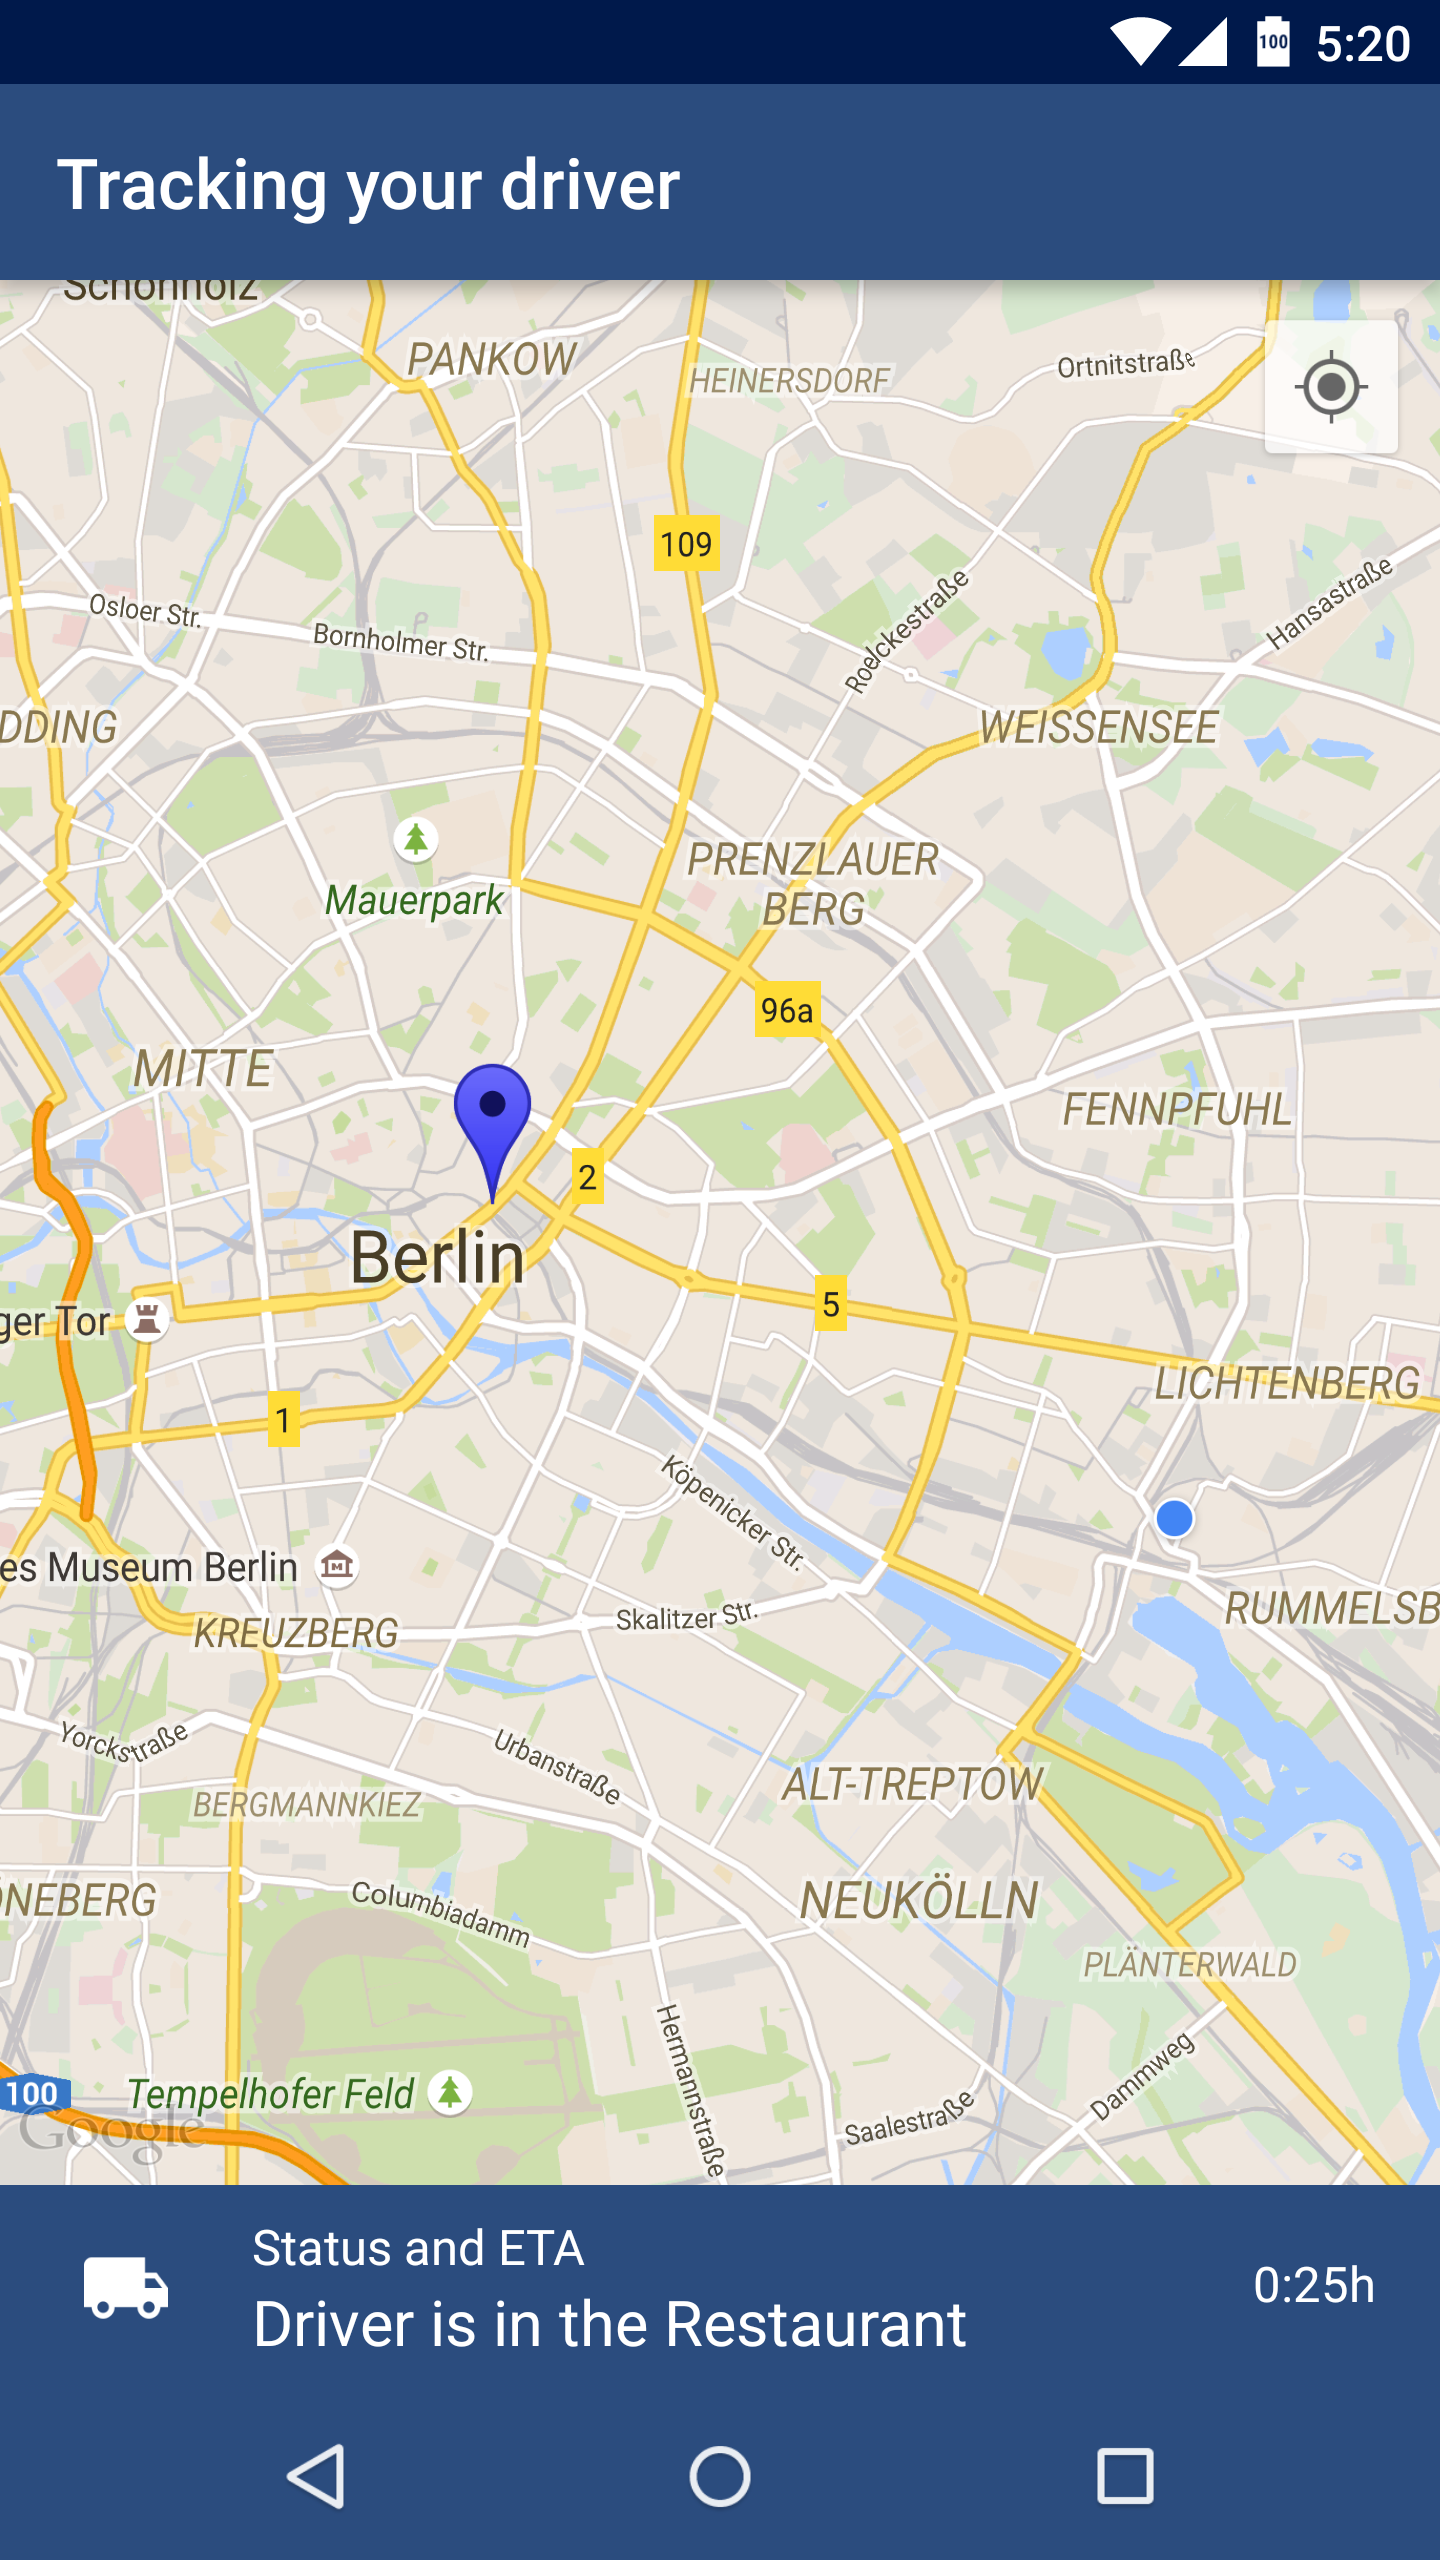
\includegraphics[width=.3\textwidth]{images/3_pickup_ended.png}\hfill
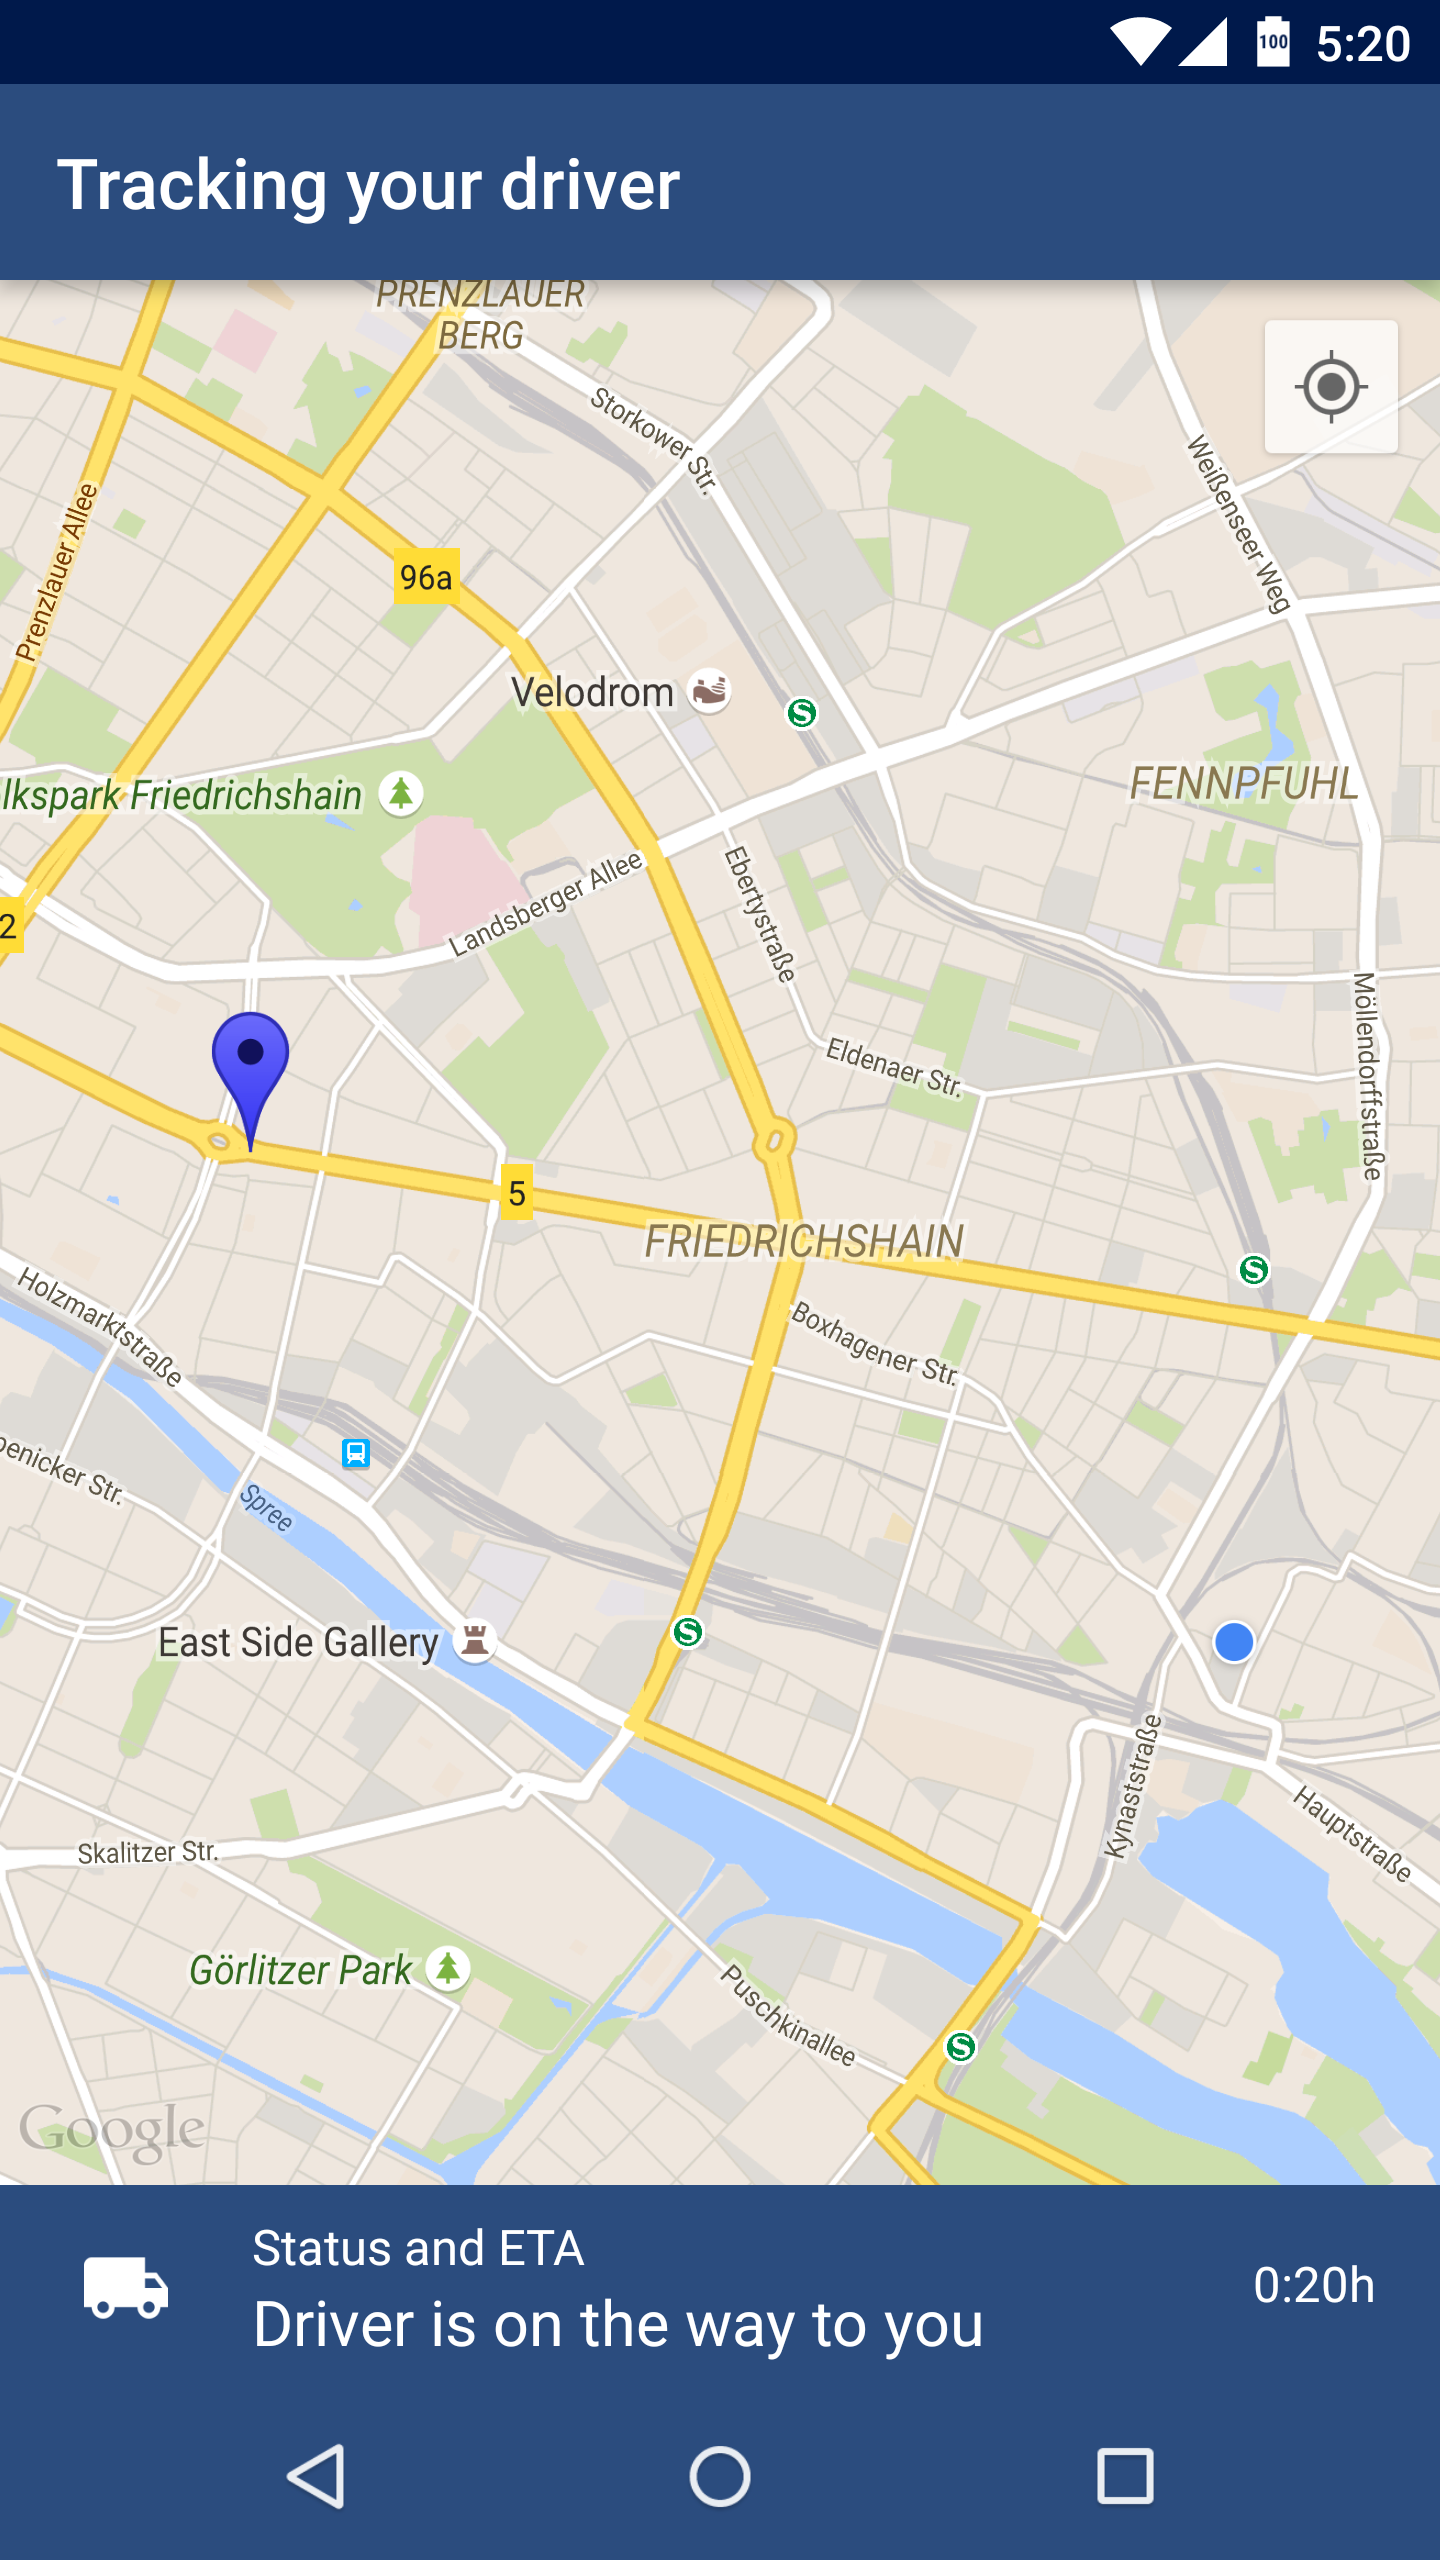
\includegraphics[width=.3\textwidth]{images/4_delivery_started.png}\hfill
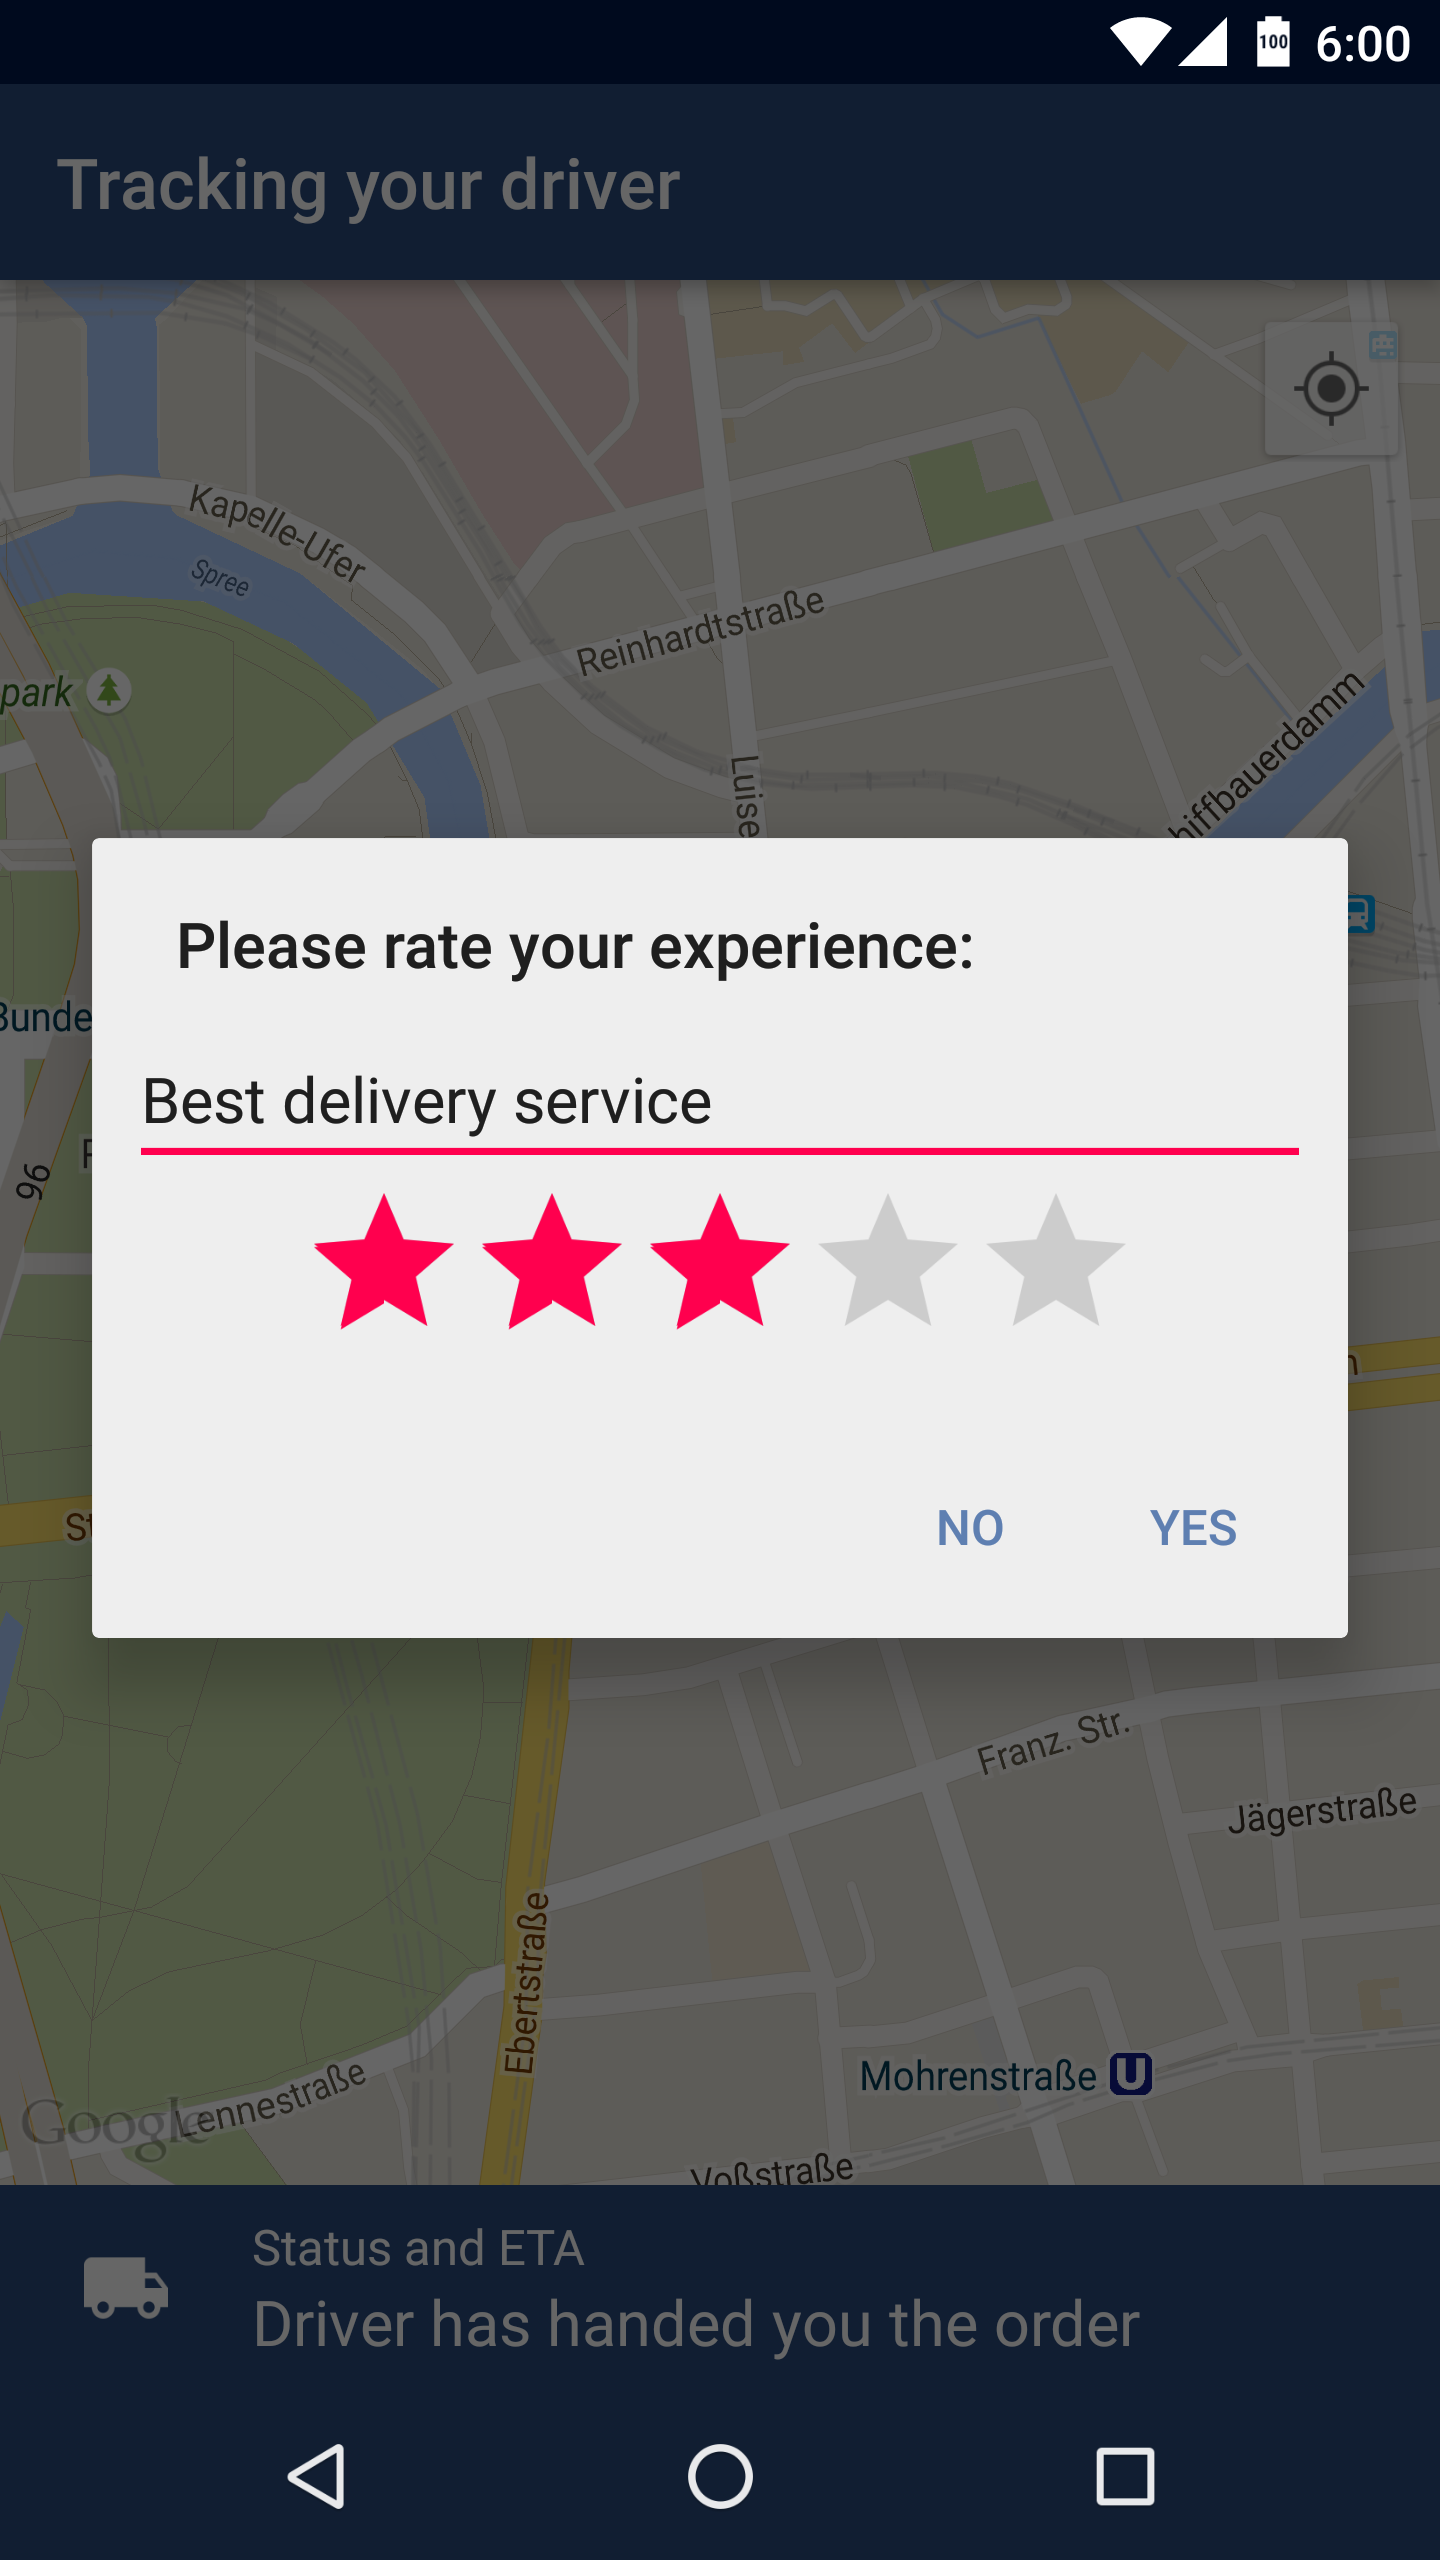
\includegraphics[width=.3\textwidth]{images/5_feedback.png}
\caption{The graphical user interface of the consumer application. When the driver is at the restaurant (left), when the driver has left the restaurant (middle) and when the driver has finished the delivery (right).}
\label{fig:consumer_application2}

\end{figure}

As soon as the driver has completed the delivery by giving the order to the customer and checking it in her driver application, a feedback dialog opens in the customer application (Figure \ref{fig:consumer_application2}, right). In this popup the customer can rate her experience and provide valuable feedback for VOLO in case something was not as she wished.\newline
After entering the feedback, the application is closed and the user is logged out from the application. The user account is now set to inactive on the server since there is nothing to track anymore. In case the user orders again, the account will be reactivated and a new password will be generated. The user receives an email with her new login credentials.\newline
This way the customer tracking application provides an easy and comfortable way of tracking an order and giving feedback about the delivery.
\newpage
\section*{Appendix Two: Code and Results}\label{section:Appendix Two: Code and Results}

The code and application will be sent by email since they contain confidential material of VOLO UG.
